\subsubsection{Wichtige Zahlenmengen}
Die natürlichen Zahlen sind jene Zahlen, die man beim Zählen verwendet:
\begin{definition}{Natürliche Zahlen}{natuerlichezahlen}
    Die Menge \(\mathbb{N}\) der natürlichen Zahlen ist die Menge
    \[ \N = \{1, 2, 3, 4, 5, \ldots\} \]
\end{definition}
Die Gemeinschaft der Mathematiker ist sich uneins, ob die Zahl \(0\) auch zu den natürlichen Zahlen gehören soll oder nicht. Bei uns wird sie standardmässig nicht dazugehören. Falls wir die Null benötigen, können wir die Zahlenmenge \(\mathbb{N}_0 = \{0, 1, 2, 3, 4, 5, \ldots\}\) betrachten.

\begin{definition}{Die ganzen Zahlen}{}
    Die Menge \(\mathbb{Z}\) der ganzen Zahlen ist definiert durch
    \[
        \mathbb{Z} = \{\ldots, -3, -2, -1, 0, 1, 2, 3, \ldots\}.
    \]

    Oder in beschreibender Form
    \[
        \mathbb{Z} = \{x \mid x \in \mathbb{N}_0 \text{ oder } -x \in \mathbb{N}\}.
    \]

    (Die beschreibende Form liest man so: \textit{\(\mathbb{Z}\) ist die Menge aller \(x\) mit der Eigenschaft, dass \(x\) in der Menge \(\mathbb{N}_0\) oder \(-x\) in der Menge \(\mathbb{N}\) liegt}.)
\end{definition}

\begin{definition}
    {Die rationale Zahlen}{}
    Das Resultat einer Division von zwei ganzen Zahlen nennt man einen (gewöhnlichen) Bruch.

    Die Menge \(\mathbb{Q}\) der rationalen Zahlen ist die Menge aller Brüche.
    \[
        \mathbb{Q}
        =
        \left\{
        \frac{a}{b}
        \;\middle|\;
        a \in \mathbb{Z}
        \text{ und }
        b \neq 0 \in \mathbb{Z}
        \right\}
    \]
\end{definition}

\textbf{Die reellen Zahlen \(\R\) }

Wenn Sie nun der Meinung sind, dass es jenseits der Brüche keine weiteren Zahlen gibt, sind Sie in bester Gesellschaft: Pythagoras (um 510 v.\,Chr. gestorben) war überzeugt, dass es gar keine anderen Zahlen als Brüche geben kann.

Als einer der Ersten hat wohl Hippasos von Metapont (ca.\ 500 v.\,Chr.) entdeckt, dass es Zahlen gibt, die sich nicht als Bruch schreiben lassen. Solche Zahlen nennt man auch \textit{irrational}. Zusammen mit den rationalen Zahlen bilden sie die Menge der reellen Zahlen:
\begin{definition}
    {Die reellen Zahlen \(\R\)}{}
    Die Menge \(\mathbb{R}\) der reellen Zahlen besteht aus allen rationalen und irrationalen Zahlen.
\end{definition}
Vielleicht haben Sie gemerkt, dass wir gar nicht genau festgelegt haben, was denn irrationale Zahlen sind. Eine genaue Definition der reellen Zahlen ist aber gar nicht so einfach. Siehe vielleicht später im Schwerpunktfach AM\dots

Wenn nichts anderes erwähnt wird, werden wir in der Mittelschule immer mit reellen Zahlen arbeiten. Diese können auf der sogenannten Zahlengerade angesiedelt werden: Jeder Zahl entspricht ein Punkt auf der Zahlengerade und umgekehrt.

\begin{center}
    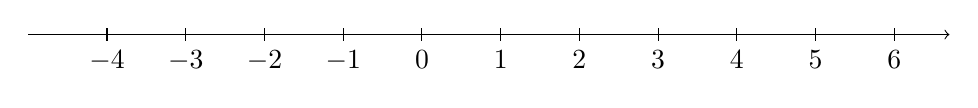
\begin{tikzpicture}
        \draw[->] (-5,0) -- (6.7,0);
        \foreach \x in {-4,-3,...,6} {
                \draw (\x,0.08) -- (\x,-0.08) node[below] {\(\x\)};
            }
    \end{tikzpicture}
\end{center}

Weitere Zahlenmengen:
\[
    \mathbb{R}^{+}
    =
    \{x \in \mathbb{R} \mid x > 0\}
    \qquad
    \text{\enquote{positive reelle Zahlen}}
\]

\[
    \mathbb{R}^{-}_{0}
    =
    \{x \in \mathbb{R} \mid x \leq 0\}
    \qquad
    \text{\enquote{negative reelle Zahlen und Null}}
\]

analog \(\mathbb{Z}^{-}\), \(\mathbb{Q}^{+}_{0}\), usw.



\textbf{\textit{Rational oder irrational?}}

Woran erkennt man eigentlich, ob eine Zahl rational ist (also in \(\mathbb{Q}\) liegt)? Das ist ganz einfach! Die Dezimaldarstellung von Brüchen ist entweder endlich oder periodisch.

\begin{itemize}
    \item \(2.423\) ist eine rationale Zahl, weil die Dezimaldarstellung endlich ist
          \[
              \left(2.423 = \frac{2423}{1000}\right).
          \]

    \item \(2.753753753753753\ldots = 2.\overline{753}\) ist eine rationale Zahl, weil die Dezimaldarstellung periodisch ist
          \[
              \left(2.\overline{753} = \frac{2751}{999}\right).
          \]
          (Wie findet man wohl den dazugehörigen Bruch?)

    \item \(1.234567891011121314\ldots\) ist eine irrationale Zahl, weil sie weder endlich noch periodisch ist.
\end{itemize}

Der letzte Punkt tönt einfacher als er ist: Schliesslich kennt man bei einer Zahl wie \(\sqrt{2}\) nicht alle unendlich vielen Ziffern nach dem Dezimalpunkt. Bloss weil sich in den ersten paar Milliarden kein sich wiederholendes Muster zeigt, heisst das noch lange nicht, dass in der darauffolgenden Unendlichkeit kein solches auftreten wird.

Mehr zu diesem Thema werden wir im letzten Teilkapitel besprechen \dots

\clearpage

\begin{ueb}
    {Übungen zu den wichtigen Zahlenmengen}{zahlenmengen}

    \begin{enumerate}
        \item Kreuzen Sie an, in welchen der angegebenen Zahlenmengen die Zahlen enthalten sind. Tipp: Wir werden später sehen, dass \(\sqrt{5}\) eine irrationale Zahl ist.

              \[
                  \begin{array}{c|c|c|c|c|c|c|c|c|c|c}
                                   & \dfrac{2}{5}   & 7               & -1.5      & -\dfrac{8}{4} & \sqrt{5} & \sqrt{16}
                                   & 1.4 \cdot 10^3 & 2.04 \cdot 10^2 & \sqrt{-5} & -\sqrt{5}                                       \\ \hline
                      \mathbb{N}   &                &                 &           &               &          &           &  &  &  & \\ \hline
                      \mathbb{Z}   &                &                 &           &               &          &           &  &  &  & \\ \hline
                      \mathbb{Q}   &                &                 &           &               &          &           &  &  &  & \\ \hline
                      \mathbb{Q}^- &                &                 &           &               &          &           &  &  &  & \\ \hline
                      \mathbb{R}   &                &                 &           &               &          &           &  &  &  &
                  \end{array}
              \]

        \item
              Beantworten Sie die Frage oder beurteilen Sie, ob die Aussage wahr oder falsch ist.

              \begin{enumerate}
                  \item Sind die negativen gewöhnlichen Brüche in \(\mathbb{Q}\) enthalten?
                  \item Jede natürliche Zahl liegt auch in \(\mathbb{Z}\).
                  \item Eine natürliche Zahl gehört nicht zu \(\mathbb{Q}\), weil sie ja schon in \(\mathbb{N}\) ist.
                  \item Liegen alle Dezimalbrüche in \(\mathbb{Q}\)?
                  \item Gehört jede Zahl in \(\mathbb{Q}\) auch zu \(\mathbb{R}\)?
              \end{enumerate}
        \item Beschreiben Sie in Worten, um welche Zahlen es sich handelt.

              \begin{enumerate}
                  \item \(\mathbb{Z}\) ohne \(\mathbb{N}\)
                  \item \(\mathbb{Z}\) ohne \(\{-1,-2,-3,\ldots\}\)
                  \item \(\mathbb{Q}^{+}\) ohne \(\{-1,-2,-3,\ldots\}\)
              \end{enumerate}
        \item Die folgenden Mengen sind in beschreibender Form angegeben. Geben Sie die Menge in aufzählender Form an.

              Zum Beispiel
              \[
                  \{n \in \mathbb{N} \mid 2n < 10\} = \{1,2,3,4\}.
              \]

              \begin{enumerate}
                  \item \(A = \{n \in \mathbb{N} \mid n \text{ ist ein Teiler von } 36\}\)
                  \item \(B = \{n \in \mathbb{N} \mid n < 10 \text{ und } n = 2k \text{ für eine Zahl } k \in \mathbb{N}\}\)
                  \item \(C = \{n \in \mathbb{N} \mid n^2 \leq 100\}\)
                  \item \(D = \{x \in \mathbb{Z} \mid -3 \leq x - 5 \leq 3\}\)
              \end{enumerate}

        \item Die folgenden Mengen sind in aufzählender Form angegeben. Geben Sie die Menge in beschreibender Form an.

              \begin{enumerate}
                  \item \(A = \{1,8,27,64,125\}\)
                  \item \(B = \{3,4,5,6,7,8,9,10\}\)
                  \item \(C = \{1,3,5,7,9,11\}\)
                  \item \(D = \{1,2,3,4,6,12\}\)
              \end{enumerate}
        \item Challenge:
              \begin{enumerate}
                  \item Erklären Sie, wie man den Bruch für die Zahl \(x = 2.\overline{753}\) findet. Tipp: Betrachten Sie die Zahl \(1000\cdot x\) und die Zahl \(x\) und berechnen Sie damit die Zahl \(999\cdot x\).
                  \item Finden Sie einen Bruch für die Zahl \(x = 1.234\overline{34}\).
              \end{enumerate}
    \end{enumerate}


\end{ueb}



% \clearpage
\emph{Lösungen:}

\begin{enumerate}
    \item
          \[
              \begin{array}{c|c|c|c|c|c|c|c|c|c|c}
                               & \dfrac{2}{5}   & 7               & -1.5      & -\dfrac{8}{4} & \sqrt{5} & \sqrt{16}
                               & 1.4 \cdot 10^3 & 2.04 \cdot 10^2 & \sqrt{-5} & -\sqrt{5}                            \\ \hline
                  \mathbb{N}   &                & \times          &           &               &          & \times
                               & \times         & \times          &           &                                      \\ \hline
                  \mathbb{Z}   &                & \times          &           & \times        &          & \times
                               & \times         & \times          &           &                                      \\ \hline
                  \mathbb{Q}   & \times         & \times          & \times    & \times        &          & \times
                               & \times         & \times          &           &                                      \\ \hline
                  \mathbb{Q}^- &                &                 & \times    & \times        &          &
                               &                &                 &           &                                      \\ \hline
                  \mathbb{R}   & \times         & \times          & \times    & \times        & \times   & \times
                               & \times         & \times          &           & \times
              \end{array}
          \]

    \item
          \begin{enumerate}
              \item Ja.
              \item Wahr.
              \item Falsch.
              \item Wahr.
              \item Ja.
          \end{enumerate}

    \item
          \begin{enumerate}
              \item Die ganzen Zahlen kleiner oder gleich \(0\).
              \item Die nichtnegativen ganzen Zahlen, also \(\mathbb{N}_0\).
              \item Die positiven rationalen Zahlen, also \(\mathbb{Q}^+\).
          \end{enumerate}

    \item
          \begin{enumerate}
              \item \(A = \{1,2,3,4,6,9,12,18,36\}\)
              \item \(B = \{2,4,6,8\}\)
              \item \(C = \{1,2,3,4,5,6,7,8,9,10\}\)
              \item \(D = \{2,3,4,5,6,7,8\}\)
          \end{enumerate}

    \item
          \begin{enumerate}
              \item \(A = \{n^3 \mid n \in \mathbb{N},\ n \leq 5\}\)
              \item \(B = \{n \in \mathbb{N} \mid 3 \leq n \leq 10\}\)
              \item \(C = \{n \in \mathbb{N} \mid n < 12 \text{ und } n \text{ ungerade}\}\)
              \item \(D = \{n \in \mathbb{N} \mid n \text{ ist ein Teiler von } 12\}\)
          \end{enumerate}

    \item \begin{enumerate}
              \item \(\frac{917}{333}\)
              \item \(\frac{611}{495}\)
          \end{enumerate}
          %       \begin{enumerate}
          %           \item
          %                 \[
          %                     1000x = 2753.\overline{753},
          %                     \qquad
          %                     x = 2.\overline{753}
          %                 \]
          %                 \[
          %                     999x = 2751
          %                     \qquad\Longrightarrow\qquad
          %                     x = \frac{2751}{999}
          %                     = \frac{917}{333}.
          %                 \]

          %           \item
          %                 \[
          %                     100000x - 1000x = 122200
          %                 \]
          %                 \[
          %                     99000x = 122200
          %                     \qquad\Longrightarrow\qquad
          %                     x = \frac{122200}{99000}
          %                     = \frac{611}{495}.
          %                 \]
          % \end{enumerate}
\end{enumerate}


